% Created by tikzDevice version 0.12.6 on 2025-04-07 11:17:48
% !TEX encoding = UTF-8 Unicode
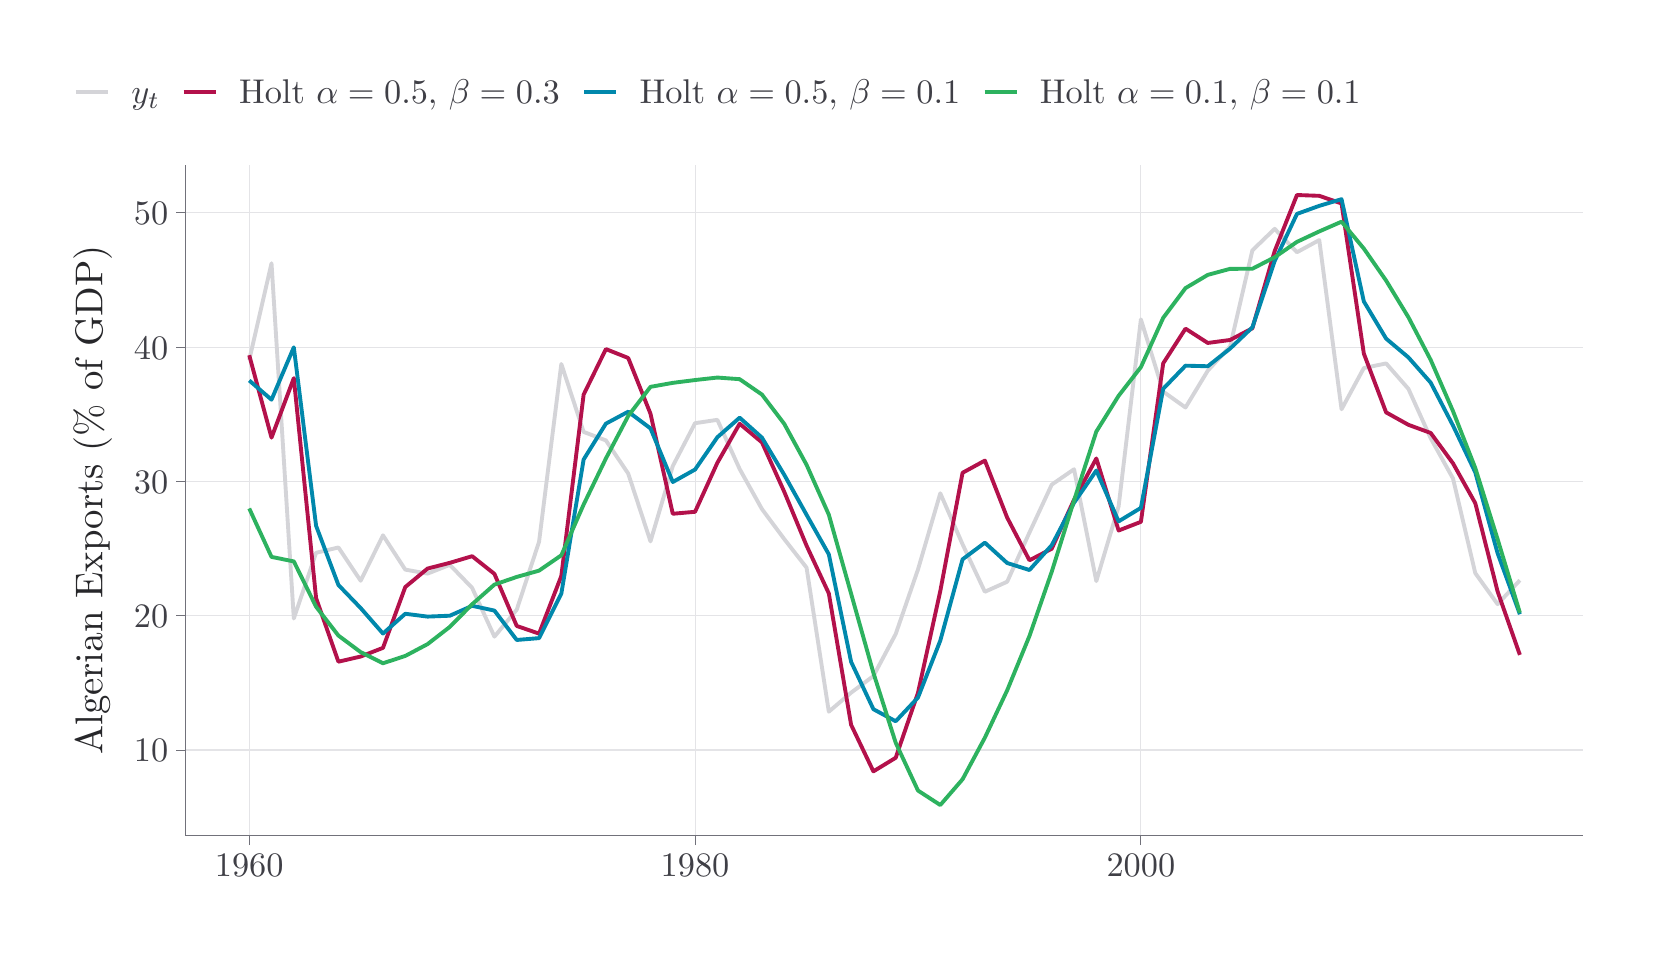
\begin{tikzpicture}[x=1pt,y=1pt]
\definecolor{fillColor}{RGB}{255,255,255}
\path[use as bounding box,fill=fillColor] (0,0) rectangle (578.16,325.21);
\begin{scope}
\path[clip] (  0.00,  0.00) rectangle (578.16,325.21);
\definecolor{drawColor}{RGB}{255,255,255}

\path[draw=drawColor,line width= 0.7pt,line join=round,line cap=round,fill=fillColor] (  0.00,  0.00) rectangle (578.16,325.21);
\end{scope}
\begin{scope}
\path[clip] ( 57.10, 33.29) rectangle (562.16,275.76);
\definecolor{drawColor}{RGB}{255,255,255}
\definecolor{fillColor}{RGB}{255,255,255}

\path[draw=drawColor,line width= 0.7pt,line join=round,line cap=round,fill=fillColor] ( 57.10, 33.29) rectangle (562.16,275.76);
\definecolor{drawColor}{RGB}{228,228,231}

\path[draw=drawColor,line width= 0.4pt,line join=round] ( 57.10, 64.19) --
	(562.16, 64.19);

\path[draw=drawColor,line width= 0.4pt,line join=round] ( 57.10,112.71) --
	(562.16,112.71);

\path[draw=drawColor,line width= 0.4pt,line join=round] ( 57.10,161.24) --
	(562.16,161.24);

\path[draw=drawColor,line width= 0.4pt,line join=round] ( 57.10,209.76) --
	(562.16,209.76);

\path[draw=drawColor,line width= 0.4pt,line join=round] ( 57.10,258.29) --
	(562.16,258.29);

\path[draw=drawColor,line width= 0.4pt,line join=round] ( 80.06, 33.29) --
	( 80.06,275.76);

\path[draw=drawColor,line width= 0.4pt,line join=round] (241.16, 33.29) --
	(241.16,275.76);

\path[draw=drawColor,line width= 0.4pt,line join=round] (402.26, 33.29) --
	(402.26,275.76);
\definecolor{drawColor}{RGB}{212,212,216}

\path[draw=drawColor,line width= 1.4pt,line join=round] ( 80.06,205.12) --
	( 88.11,240.07) --
	( 96.17,111.71) --
	(104.22,135.45) --
	(112.28,137.38) --
	(120.33,125.35) --
	(128.39,141.76) --
	(136.44,129.38) --
	(144.50,127.93) --
	(152.55,131.10) --
	(160.61,122.77) --
	(168.66,105.16) --
	(176.72,114.89) --
	(184.78,139.42) --
	(192.83,203.69) --
	(200.89,179.14) --
	(208.94,176.06) --
	(217.00,164.09) --
	(225.05,139.58) --
	(233.11,166.81) --
	(241.16,182.29) --
	(249.22,183.50) --
	(257.27,165.73) --
	(265.33,151.25) --
	(273.38,140.42) --
	(281.44,130.10) --
	(289.49, 78.04) --
	(297.55, 84.92) --
	(305.60, 90.91) --
	(313.66,106.11) --
	(321.71,129.42) --
	(329.77,156.96) --
	(337.82,138.53) --
	(345.88,121.37) --
	(353.93,124.99) --
	(361.99,142.77) --
	(370.04,160.08) --
	(378.10,165.64) --
	(386.15,125.22) --
	(394.21,152.26) --
	(402.26,219.81) --
	(410.32,193.70) --
	(418.38,187.95) --
	(426.43,201.27) --
	(434.49,210.02) --
	(442.54,244.73) --
	(450.60,252.52) --
	(458.65,244.06) --
	(466.71,248.46) --
	(474.76,187.31) --
	(482.82,202.22) --
	(490.87,203.88) --
	(498.93,194.68) --
	(506.98,176.82) --
	(515.04,162.30) --
	(523.09,128.10) --
	(531.15,116.89) --
	(539.20,125.52);
\definecolor{drawColor}{RGB}{179,17,75}

\path[draw=drawColor,line width= 1.4pt,line join=round] ( 80.06,206.85) --
	( 88.11,177.07) --
	( 96.17,198.56) --
	(104.22,119.07) --
	(112.28, 96.10) --
	(120.33, 97.97) --
	(128.39,101.10) --
	(136.44,123.07) --
	(144.50,129.76) --
	(152.55,131.83) --
	(160.61,134.23) --
	(168.66,127.83) --
	(176.72,109.02) --
	(184.78,106.25) --
	(192.83,127.07) --
	(200.89,192.61) --
	(208.94,209.06) --
	(217.00,205.85) --
	(225.05,185.72) --
	(233.11,149.56) --
	(241.16,150.27) --
	(249.22,167.98) --
	(257.27,182.09) --
	(265.33,175.35) --
	(273.38,157.51) --
	(281.44,138.05) --
	(289.49,120.78) --
	(297.55, 73.29) --
	(305.60, 56.47) --
	(313.66, 61.39) --
	(321.71, 84.87) --
	(329.77,121.63) --
	(337.82,164.37) --
	(345.88,168.78) --
	(353.93,148.18) --
	(361.99,132.74) --
	(370.04,136.92) --
	(378.10,154.61) --
	(386.15,169.54) --
	(394.21,143.51) --
	(402.26,146.64) --
	(410.32,203.92) --
	(418.38,216.45) --
	(426.43,211.28) --
	(434.49,212.36) --
	(442.54,216.57) --
	(450.60,244.48) --
	(458.65,264.74) --
	(466.71,264.44) --
	(474.76,261.69) --
	(482.82,207.43) --
	(490.87,186.19) --
	(498.93,181.70) --
	(506.98,178.75) --
	(515.04,167.77) --
	(523.09,153.38) --
	(531.15,121.50) --
	(539.20, 98.57);
\definecolor{drawColor}{RGB}{1,136,172}

\path[draw=drawColor,line width= 1.4pt,line join=round] ( 80.06,197.72) --
	( 88.11,190.78) --
	( 96.17,209.71) --
	(104.22,145.20) --
	(112.28,123.83) --
	(120.33,115.48) --
	(128.39,106.27) --
	(136.44,113.42) --
	(144.50,112.40) --
	(152.55,112.72) --
	(160.61,116.30) --
	(168.66,114.57) --
	(176.72,103.96) --
	(184.78,104.62) --
	(192.83,120.69) --
	(200.89,169.16) --
	(208.94,182.12) --
	(217.00,186.45) --
	(225.05,180.40) --
	(233.11,161.03) --
	(241.16,165.54) --
	(249.22,177.21) --
	(257.27,184.28) --
	(265.33,177.07) --
	(273.38,163.65) --
	(281.44,149.20) --
	(289.49,134.91) --
	(297.55, 96.04) --
	(305.60, 78.94) --
	(313.66, 74.58) --
	(321.71, 83.15) --
	(329.77,103.72) --
	(337.82,133.10) --
	(345.88,139.11) --
	(353.93,131.77) --
	(361.99,129.23) --
	(370.04,138.20) --
	(378.10,153.53) --
	(386.15,165.19) --
	(394.21,146.81) --
	(402.26,151.69) --
	(410.32,194.71) --
	(418.38,203.07) --
	(426.43,202.86) --
	(434.49,209.25) --
	(442.54,216.91) --
	(450.60,240.87) --
	(458.65,257.91) --
	(466.71,260.82) --
	(474.76,263.23) --
	(482.82,226.27) --
	(490.87,212.84) --
	(498.93,206.06) --
	(506.98,196.93) --
	(515.04,181.42) --
	(523.09,164.50) --
	(531.15,135.30) --
	(539.20,113.25);
\definecolor{drawColor}{RGB}{45,178,95}

\path[draw=drawColor,line width= 1.4pt,line join=round] ( 80.06,151.47) --
	( 88.11,133.97) --
	( 96.17,132.34) --
	(104.22,115.96) --
	(112.28,105.55) --
	(120.33, 99.56) --
	(128.39, 95.54) --
	(136.44, 98.18) --
	(144.50,102.45) --
	(152.55,108.69) --
	(160.61,116.86) --
	(168.66,123.97) --
	(176.72,126.73) --
	(184.78,129.01) --
	(192.83,134.55) --
	(200.89,152.88) --
	(208.94,169.54) --
	(217.00,184.89) --
	(225.05,195.42) --
	(233.11,196.86) --
	(241.16,197.88) --
	(249.22,198.78) --
	(257.27,198.19) --
	(265.33,192.63) --
	(273.38,182.05) --
	(281.44,167.27) --
	(289.49,149.23) --
	(297.55,120.66) --
	(305.60, 92.07) --
	(313.66, 66.81) --
	(321.71, 49.54) --
	(329.77, 44.31) --
	(337.82, 53.62) --
	(345.88, 68.65) --
	(353.93, 85.73) --
	(361.99,105.39) --
	(370.04,128.61) --
	(378.10,154.37) --
	(386.15,179.25) --
	(394.21,192.19) --
	(402.26,202.55) --
	(410.32,220.35) --
	(418.38,231.10) --
	(426.43,235.88) --
	(434.49,238.06) --
	(442.54,238.09) --
	(450.60,242.25) --
	(458.65,247.80) --
	(466.71,251.58) --
	(474.76,255.10) --
	(482.82,245.38) --
	(490.87,233.81) --
	(498.93,220.56) --
	(506.98,205.14) --
	(515.04,186.63) --
	(523.09,166.09) --
	(531.15,140.39) --
	(539.20,113.79);
\end{scope}
\begin{scope}
\path[clip] (  0.00,  0.00) rectangle (578.16,325.21);
\definecolor{drawColor}{RGB}{113,113,122}

\path[draw=drawColor,line width= 0.3pt,line join=round] ( 57.10, 33.29) --
	( 57.10,275.76);
\end{scope}
\begin{scope}
\path[clip] (  0.00,  0.00) rectangle (578.16,325.21);
\definecolor{drawColor}{RGB}{63,63,70}

\node[text=drawColor,anchor=base east,inner sep=0pt, outer sep=0pt, scale=  1.24] at ( 50.80, 59.90) {10};

\node[text=drawColor,anchor=base east,inner sep=0pt, outer sep=0pt, scale=  1.24] at ( 50.80,108.43) {20};

\node[text=drawColor,anchor=base east,inner sep=0pt, outer sep=0pt, scale=  1.24] at ( 50.80,156.96) {30};

\node[text=drawColor,anchor=base east,inner sep=0pt, outer sep=0pt, scale=  1.24] at ( 50.80,205.48) {40};

\node[text=drawColor,anchor=base east,inner sep=0pt, outer sep=0pt, scale=  1.24] at ( 50.80,254.01) {50};
\end{scope}
\begin{scope}
\path[clip] (  0.00,  0.00) rectangle (578.16,325.21);
\definecolor{drawColor}{RGB}{113,113,122}

\path[draw=drawColor,line width= 0.3pt,line join=round] ( 53.60, 64.19) --
	( 57.10, 64.19);

\path[draw=drawColor,line width= 0.3pt,line join=round] ( 53.60,112.71) --
	( 57.10,112.71);

\path[draw=drawColor,line width= 0.3pt,line join=round] ( 53.60,161.24) --
	( 57.10,161.24);

\path[draw=drawColor,line width= 0.3pt,line join=round] ( 53.60,209.76) --
	( 57.10,209.76);

\path[draw=drawColor,line width= 0.3pt,line join=round] ( 53.60,258.29) --
	( 57.10,258.29);
\end{scope}
\begin{scope}
\path[clip] (  0.00,  0.00) rectangle (578.16,325.21);
\definecolor{drawColor}{RGB}{113,113,122}

\path[draw=drawColor,line width= 0.3pt,line join=round] ( 57.10, 33.29) --
	(562.16, 33.29);
\end{scope}
\begin{scope}
\path[clip] (  0.00,  0.00) rectangle (578.16,325.21);
\definecolor{drawColor}{RGB}{113,113,122}

\path[draw=drawColor,line width= 0.3pt,line join=round] ( 80.06, 29.79) --
	( 80.06, 33.29);

\path[draw=drawColor,line width= 0.3pt,line join=round] (241.16, 29.79) --
	(241.16, 33.29);

\path[draw=drawColor,line width= 0.3pt,line join=round] (402.26, 29.79) --
	(402.26, 33.29);
\end{scope}
\begin{scope}
\path[clip] (  0.00,  0.00) rectangle (578.16,325.21);
\definecolor{drawColor}{RGB}{63,63,70}

\node[text=drawColor,anchor=base,inner sep=0pt, outer sep=0pt, scale=  1.24] at ( 80.06, 18.42) {1960};

\node[text=drawColor,anchor=base,inner sep=0pt, outer sep=0pt, scale=  1.24] at (241.16, 18.42) {1980};

\node[text=drawColor,anchor=base,inner sep=0pt, outer sep=0pt, scale=  1.24] at (402.26, 18.42) {2000};
\end{scope}
\begin{scope}
\path[clip] (  0.00,  0.00) rectangle (578.16,325.21);
\definecolor{drawColor}{RGB}{39,39,42}

\node[text=drawColor,rotate= 90.00,anchor=base,inner sep=0pt, outer sep=0pt, scale=  1.40] at ( 27.00,154.52) {Algerian Exports (\% of GDP)};
\end{scope}
\begin{scope}
\path[clip] (  0.00,  0.00) rectangle (578.16,325.21);
\definecolor{drawColor}{RGB}{255,255,255}
\definecolor{fillColor}{RGB}{255,255,255}

\path[draw=drawColor,line width= 0.7pt,line join=round,line cap=round,fill=fillColor] ( 16.00,289.76) rectangle (482.03,309.22);
\end{scope}
\begin{scope}
\path[clip] (  0.00,  0.00) rectangle (578.16,325.21);
\definecolor{drawColor}{RGB}{255,255,255}
\definecolor{fillColor}{RGB}{255,255,255}

\path[draw=drawColor,line width= 0.7pt,line join=round,line cap=round,fill=fillColor] ( 16.00,294.76) rectangle ( 30.45,309.22);
\end{scope}
\begin{scope}
\path[clip] (  0.00,  0.00) rectangle (578.16,325.21);
\definecolor{drawColor}{RGB}{212,212,216}

\path[draw=drawColor,line width= 1.4pt,line join=round] ( 17.45,301.99) -- ( 29.01,301.99);
\end{scope}
\begin{scope}
\path[clip] (  0.00,  0.00) rectangle (578.16,325.21);
\definecolor{drawColor}{RGB}{255,255,255}
\definecolor{fillColor}{RGB}{255,255,255}

\path[draw=drawColor,line width= 0.7pt,line join=round,line cap=round,fill=fillColor] ( 54.93,294.76) rectangle ( 69.39,309.22);
\end{scope}
\begin{scope}
\path[clip] (  0.00,  0.00) rectangle (578.16,325.21);
\definecolor{drawColor}{RGB}{179,17,75}

\path[draw=drawColor,line width= 1.4pt,line join=round] ( 56.38,301.99) -- ( 67.94,301.99);
\end{scope}
\begin{scope}
\path[clip] (  0.00,  0.00) rectangle (578.16,325.21);
\definecolor{drawColor}{RGB}{255,255,255}
\definecolor{fillColor}{RGB}{255,255,255}

\path[draw=drawColor,line width= 0.7pt,line join=round,line cap=round,fill=fillColor] (199.63,294.76) rectangle (214.09,309.22);
\end{scope}
\begin{scope}
\path[clip] (  0.00,  0.00) rectangle (578.16,325.21);
\definecolor{drawColor}{RGB}{1,136,172}

\path[draw=drawColor,line width= 1.4pt,line join=round] (201.08,301.99) -- (212.64,301.99);
\end{scope}
\begin{scope}
\path[clip] (  0.00,  0.00) rectangle (578.16,325.21);
\definecolor{drawColor}{RGB}{255,255,255}
\definecolor{fillColor}{RGB}{255,255,255}

\path[draw=drawColor,line width= 0.7pt,line join=round,line cap=round,fill=fillColor] (344.33,294.76) rectangle (358.78,309.22);
\end{scope}
\begin{scope}
\path[clip] (  0.00,  0.00) rectangle (578.16,325.21);
\definecolor{drawColor}{RGB}{45,178,95}

\path[draw=drawColor,line width= 1.4pt,line join=round] (345.78,301.99) -- (357.34,301.99);
\end{scope}
\begin{scope}
\path[clip] (  0.00,  0.00) rectangle (578.16,325.21);
\definecolor{drawColor}{RGB}{63,63,70}

\node[text=drawColor,anchor=base west,inner sep=0pt, outer sep=0pt, scale=  1.24] at ( 37.45,297.70) {$y_t$};
\end{scope}
\begin{scope}
\path[clip] (  0.00,  0.00) rectangle (578.16,325.21);
\definecolor{drawColor}{RGB}{63,63,70}

\node[text=drawColor,anchor=base west,inner sep=0pt, outer sep=0pt, scale=  1.24] at ( 76.39,297.70) {Holt $\alpha = 0.5$, $\beta = 0.3$};
\end{scope}
\begin{scope}
\path[clip] (  0.00,  0.00) rectangle (578.16,325.21);
\definecolor{drawColor}{RGB}{63,63,70}

\node[text=drawColor,anchor=base west,inner sep=0pt, outer sep=0pt, scale=  1.24] at (221.09,297.70) {Holt $\alpha = 0.5$, $\beta = 0.1$};
\end{scope}
\begin{scope}
\path[clip] (  0.00,  0.00) rectangle (578.16,325.21);
\definecolor{drawColor}{RGB}{63,63,70}

\node[text=drawColor,anchor=base west,inner sep=0pt, outer sep=0pt, scale=  1.24] at (365.78,297.70) {Holt $\alpha = 0.1$, $\beta = 0.1$};
\end{scope}
\end{tikzpicture}
